\section{Continuity}
    We now discuss continuity, uniform continuity, and related theorems.
    \begin{definition}
        A function $f:S\rightarrow\mathbb{R}$ on a subset
        $S\subseteq\mathbb{R}$ continuous at a point $x\in{S}$ is a function
        such that for all $\varepsilon>0$ there is a $\delta>0$ such that for
        all $x_{0}\in{S}$, $|x-x_{0}|<\delta$ implies
        $|f(x)-f(x_{0})|<\varepsilon$. That is:
        \begin{equation}
            \forall_{\varepsilon>0}\exists_{\delta>0}:
            x\in{S},|x-x_{0}|<\delta
            \Rightarrow|f(x)-f(x_{0})|<\varepsilon
        \end{equation}
    \end{definition}
    \begin{theorem}
        If $S\subseteq\mathbb{R}$, $x\in{S}$, $f:S\rightarrow\mathbb{R}$ is
        continuous at $x$, and if $a:\mathbb{N}\rightarrow{S}$ is a convergent
        sequence such that $a_{n}\rightarrow{x}$, then
        $f(a_{n})\rightarrow{f(x)}$.
    \end{theorem}
    \begin{proof}
        For let $\varepsilon>0$. As $f$ is continuous there is a $\delta>0$
        such that, for all $x_{0}\in{S}$ such that $|x-x_{0}|<\delta$,
        $|f(x)-f(x_{0})|<\varepsilon$. But $a_{n}\rightarrow{x}$, and thus
        there is an $N\in\mathbb{N}$ such that, for all $n>N$,
        $|x-a_{n}|<\delta$. But then, for all $n>N$,
        $|f(x)-f(a_{n})|<\varepsilon$. Therefore, $f(a_{n})\rightarrow{f(x)}$.
    \end{proof}
    The converse of this theorem is true, giving us
    an equivalent definition of continuity.
    \begin{theorem}
        If $S\subseteq\mathbb{R}$, $x\in{S}$ and $f:S\rightarrow\mathbb{R}$
        is a function such that for all sequences
        $a:\mathbb{N}\rightarrow\mathbb{R}$ such that $a_{n}\rightarrow{x}$,
        $f(a_{n})\rightarrow{f(x)}$, then $f$ is continuous at $x$.
    \end{theorem}
    \begin{proof}
        For suppose not. Then there is an $\varepsilon>0$ such that, for all
        $\delta>0$, there is an $x_{0}\in{S}$ such that $|x-x_{0}|<\delta$ and
        $|f(x)-f(x_{0})|\geq\varepsilon$. 
        Let $a:\mathbb{N}\rightarrow\mathbb{R}$ be a sequence such that, for
        all $n\in\mathbb{N}$, $|a_{n}-x|<1/n$, but
        $|f(x)-f(a_{n})|\geq\varepsilon$. But then $a_{n}\rightarrow{x}$. But
        for all sequences $a$ such that $a_{n}\rightarrow{x}$,
        $f(a_{n})\rightarrow{f(x)}$. But, for all $n$,
        $|f(x)-f(a_{n})|\geq\varepsilon$, a contradiction.
        Therefore, $f$ is continuous at $x$.
    \end{proof}
    \begin{theorem}
        If $x\in\mathbb{R}$ and $a:\mathbb{N}\rightarrow\mathbb{R}$ is a
        convergent sequence such that $a_{n}\rightarrow{x}$ and for all
        $n\in\mathbb{N}$, $a_{n}\geq{0}$, then $x\geq{0}$.
    \end{theorem}
    \begin{proof}
        For suppose not. Suppose $x<0$. Let $\varepsilon=|x|/2$. Then, as
        $\varepsilon>0$, there is an $N\in\mathbb{N}$ such that for all $n>N$,
        $|x-a_{n}|<\varepsilon$. But then $a_{N+1}<x+\varepsilon=x/2<0$, a
        contradiction as $a_{N+1}\geq{0}$.
    \end{proof}
    \begin{theorem}
        \label{thm:Continuous_Limit_of_Pos_Sequ_is_nonneg}
        If $S\subseteq\mathbb{R}$, $x\in{S}$, $f:S\rightarrow\mathbb{R}$ is
        continuous at $x$, and if $a:\mathbb{N}\rightarrow\mathbb{R}$ is a
        sequence such that  $a_{n}\rightarrow{x}$ and $f(a_{n})>0$
        for all $n\in\mathbb{N}$, then $f(x)\geq{0}$.
    \end{theorem}
    \begin{proof}
        For suppose not. Let $r=f(x)<0$, and let $\varepsilon=|r|/2$. Then
        $\varepsilon>0$. But from continuity, there is a $\delta>0$ such that
        for all $x_{0}\in{S}$ such that $|x-x_{0}|<\delta$,
        $|f(x)-f(x_{0})|<\varepsilon$. But $a_{n}\rightarrow{x}$, and thus
        there is an $N\in\mathbb{N}$ such that for all $n>N$,
        $|x-a_{n}|<\delta$. Thus $|f(x)-f(a_{N+1})|<\varepsilon$. But then
        $f(a_{n})<f(x)+\varepsilon=f(x)/2<0$, a contradiction as
        $f(a_{N+1})>0$. Therefore, etc.
    \end{proof}
    \begin{theorem}
        If $x\in\mathbb{R}$, $f:\mathbb{R}\rightarrow\mathbb{R}$ is continuous
        at $x$, and if $f(x)>0$, then there is an open interval $\mathcal{U}$
        such that $x\in\mathcal{U}$, and for all $y\in\mathcal{U}$, $f(y)>0$.
    \end{theorem}
    \begin{proof}
        For let $\varepsilon=f(x)/2$. Then $\varepsilon>0$, and thus there is a
        $\delta>0$ such that for all $x_{0}\in\mathbb{R}$ such that
        $|x-x_{0}|<\delta$, $|f(x)-f(x_{0})|<\varepsilon$. Let
        $\mathcal{U}=(x-\delta,x+\delta)$. Then $\mathcal{U}$ is an open
        intervals and if $y\in\mathcal{U}$, then $|x-y|<\delta$, and therefore:
        \begin{equation}
            |f(y)-f(x)|<\varepsilon
            \Rightarrow
            f(y)>f(x)-\varepsilon
            =\frac{f(x)}{2}>0
        \end{equation}
        Thus, for all $y\in\mathcal{U}$, $f(y)>0$.
    \end{proof}
    \begin{definition}
        A continuous function on $S\subseteq\mathbb{R}$ is a function
        $f:S\rightarrow\mathbb{R}$ such that $f$ is continuous at all
        $x\in{S}$. That is:
        \begin{equation}
            \forall_{x\in{S}}\forall_{\varepsilon>0}
            \exists_{\delta>0}:x_{0}\in{S},|x-x_{0}|<\delta
            \Rightarrow|f(x)-f(x_{0})|<\varepsilon
        \end{equation}
    \end{definition}
    This definition comes from the fact that continuity is a point-wise
    property, and not a ``curve'' property. Continuous functions are
    functions that have point-wise continuity at every point. The statement
    ``A continuous function is a curve that you can draw,'' which many have
    heard in calculus, is slightly misleading. There are functions that are
    continuous at one point and nowhere else. There are functions that are
    continuous on the irrationals and discontinuous on the rationals. For
    example, if $x$ is rational write it as $x=p/q$ where $p$ and $q$ are
    integers and relatively prime. Define $f$ as follows:
    \begin{equation}
        f(x)=
        \begin{cases}
            \frac{1}{q},&x\in\mathbb{Q}\\
            0,&x\notin\mathbb{Q}
        \end{cases}
    \end{equation}
    This function, which is known as Dirichlet's Function, but also as the
    Popcorn Function, or Thomae's Function, is continuous at every irrational
    number and discontinuous at every rational number.
    \begin{figure}[H]
        \captionsetup{type=figure}
        \centering
        \documentclass[crop,class=article]{standalone}
%----------------------------Preamble-------------------------------%
\usepackage{tikz}                       % Drawing/graphing tools.
\usetikzlibrary{arrows.meta}            % Latex arrows.
%--------------------------Main Document----------------------------%
\begin{document}
    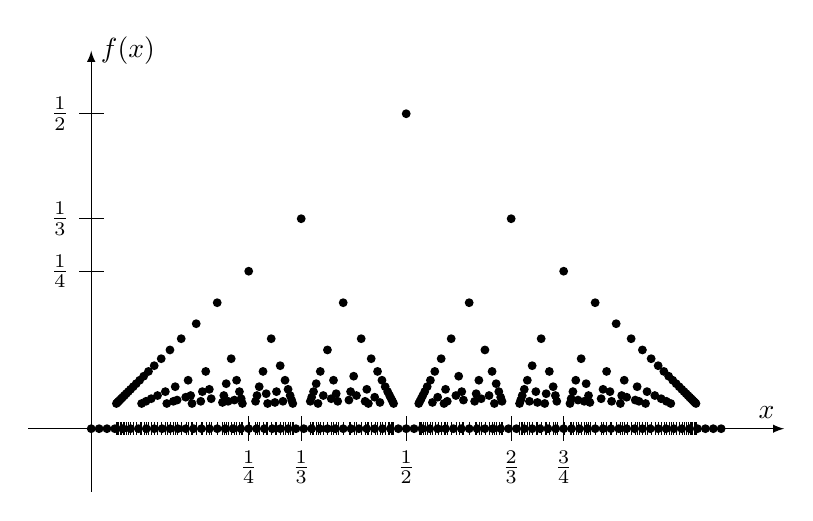
\begin{tikzpicture}[scale=8,>=latex]
        \draw[->] (-0.1,0) -- (1.1,0)
            node[above left] {$x$};
        \draw[->] (0,-0.1) -- (0,0.6)
            node[right] {$f(x)$};
        \draw (0.02,1/2) -- (-0.02,1/2)
            node[left]{$\frac{1}{2}$};
        \draw (0.02,1/3) -- (-0.02,1/3)
            node[left]{$\frac{1}{3}$};
        \draw (0.02,1/4) -- (-0.02,1/4)
            node[left]{$\frac{1}{4}$};
        \foreach\X[%
            evaluate=\X as \Ymax using {int(\X-1)}]
            in {25,24,...,2}{%
                \foreach\Y in {1,...,\Ymax}{%
                    \ifnum\X<5
                        \draw
                        (\Y/\X,0.02) -- (\Y/\X,-0.02)
                        node[below,fill=white]
                            {$\frac{\Y}{\X}$};
                    \else
                        \draw[ultra thin]
                        (\Y/\X,0.01) to (\Y/\X,-0.01);
                    \fi
                    \pgfmathtruncatemacro{\TST}
                        {gcd(\X,\Y)}
                    \ifnum\TST=1
                        \fill ({\Y/\X},1/\X) 
                            circle (0.2pt); 
                    \fi
                }
        }
        \foreach\X in {0,1,...,80}
        {\fill (\X/80,0) circle(0.2pt);}
    \end{tikzpicture}
\end{document}
        \caption[Dirichlet's Function]
            {Dirichlet's Function is Continuous on
             $\mathbb{R}\setminus\mathbb{Q}$ and
             Discontinuous on $\mathbb{Q}$}
        \label{fig:Funct:Dirichlet_Thomae_Function}
    \end{figure}
    There is no ``reverse,'' of this function. That is, there is no function
    which is continuous on $\mathbb{Q}$ and discontinuous at every irrational
    number. Uniform continuity is a property of all points in the domain of a
    function. Point-wise continuity says that given a point $x$ and a positive
    number $\varepsilon$, one can find a $\delta$ satisfying a certain
    property. The key part is that the point $x$ must be specified first. That
    is, the $\delta$ may be dependent on $x$. Uniform continuity occurs when a
    $\delta>0$ can be chosen regardless of $x$. $\delta$ is only dependent on
    $\varepsilon$.
    \begin{definition}
        A uniformly continuous function on a subset $S\subseteq\mathbb{R}$
        is a function $f:S\rightarrow\mathbb{R}$ such that:
        \begin{equation*}
            \forall_{\varepsilon>0}\exists_{\delta>0}
            \forall_{x\in{S}}:\forall_{x_{0}\in{S}},|x-x_{0}|<\delta
            \Rightarrow|f(x)-f(x_{0})|<\varepsilon    
        \end{equation*}
    \end{definition}
    Continuity is a point-wise property. There are functions that are
    continuous at one point and nowhere else. Uniform continuity, however, is a
    set property. You can't have uniform continuity at a single point, but
    rather on a set of points. Unless, of course, your domain $S$ is a single
    point. But that's rather boring.
    \begin{theorem}
        \label{thm:Equiv_Def_of_Uni_Cont}%
        A function $f:S\rightarrow\mathbb{R}$ is uniformly continuous if and
        only if for all sequences $x,y:\mathbb{N}\rightarrow\mathbb{R}$ such
        that $x_{n}-y_{n}\rightarrow{0}$, $f(x_{n})-f(y_{n})\rightarrow{0}$.
    \end{theorem}
    \begin{proof}
        Let $\varepsilon>0$. If $f$ is uniformly continuous, then there is a
        $\delta>0$ such that for all $x$, $x_{0}\in{S}$ such that
        $|x-x_{0}|<\delta$, we have that $|f(x)-f(x_{0})|<\varepsilon$. But
        if $x_{n}-y_{n}\rightarrow{0}$, then there is an $N\in\mathbb{N}$ such
        that for all $n>N$, $|x_{n}-y_{n}|<\delta$. But then, for all $n>N$,
        $|f(x_{n})-f(y_{n})|<\varepsilon$. Therefore,
        $f(x_{n})-f(y_{n})\rightarrow{0}$. Proving the converse, suppose not.
        If $f$ is not uniformly continuous, then there exists $\varepsilon>0$
        such that for all $\delta>0$ there exists $x$, $x_{0}\in{S}$ such that
        $|x-x_{0}|<\delta$ and yet $|f(x)-f(x_{0})|\geq{\varepsilon}$. Let
        $x_{n}$ and $y_{n}$ be points such that $|x_{n}-y_{n}|<\frac{1}{n}$ and
        yet $|f(x_{n})-f(y_{n})|\geq\varepsilon$. Then
        $x_{n}-y_{n}\rightarrow{0}$. But if $x_{n}-y_{n}\rightarrow{0}$, then
        $f(x_{n})-f(y_{n})\rightarrow{0}$. But for all $n$,
        $|f(x_{n})-f(y_{n})|\geq{\varepsilon}$, a contradiction.
    \end{proof}
    The requirement of uniform continuity is crucial. Let
    $f:(0,1)\rightarrow\mathbb{R}$ be defined by $f(x)=x^{-1}$. Then $f$ is
    continuous, but not uniformly continuous. Let $x_{n}=n^{-1}$ and
    $y_{n}=2n^{-1}$. Then $|y_{n}-x_{n}|=n^{-1}\rightarrow{0}$, but
    $|f(y_{n})-f(x_{n})|=n/2$, which diverges. Point-wise continuity says
    $f(x_{n})-f(x)\rightarrow{0}$, whereas uniform continuity allows the target
    to vary as well. Point-wise continuity can not guarantee this. The set
    under consideration is also crucial to uniform continuity. Indeed, the
    function $f(x)=x^{-1}$ \textit{is} uniformly continuous on $(1,\infty)$.
    For if $x,y\in(1,\infty)$:
    \begin{equation}
        |f(x)-f(y)|=\Big|\frac{1}{x}-\frac{1}{y}\Big|
                   =\Big|\frac{x-y}{xy}\Big|\leq|x-y|
    \end{equation}
    Choosing $\delta=\varepsilon/2$ gives the result.
    \begin{theorem}
        \label{thm:Cont_on_Closed_Interval_Is_Uni_Cont}%
        If $f:[a,b]\rightarrow\mathbb{R}$ is continuous,
        then $f$ is uniformly continuous.
    \end{theorem}
    \begin{proof}
        Suppose not. Then, by Thm.~\ref{thm:Equiv_Def_of_Uni_Cont},
        there are sequences $x,y:\mathbb{N}\rightarrow[a,b]$ such that
        $x_{n}-y_{n}\rightarrow{0}$, yet there is an $\varepsilon>0$ such that,
        for all $N\in\mathbb{N}$, there is an $n>N$ such that
        $|f(x_{n})-f(y_{n})|\geq\varepsilon$. Let
        $k:\mathbb{N}\rightarrow\mathbb{N}$ be a subsequence such that, for all
        $n\in\mathbb{N}$, $|f(x_{k_{n}})-f(y_{k_{n}})|\geq\varepsilon$. By the
        Bolzano-Weierstrass theorem there is a convergent subsequence
        $j:\mathbb{N}\rightarrow\mathbb{N}$ of $x\circ{k}$. Let $\alpha$
        be the limit. But for all $n\in\mathbb{N}$:
        \begin{subequations}
            \begin{equation}
                y_{j_{k_n}}=x_{j_{k_{n}}}-(y_{j_{k_{n}}}-x_{j_{k_{n}}})
                \Rightarrow
                y_{j_{k_{n}}}\rightarrow\alpha
            \end{equation}
            Let $X,Y:\mathbb{N}\rightarrow[a,b]$ be sequences defined by
            $X_{n}=x_{j_{k_{n}}}$ and $Y_{n}=y_{j_{k_{n}}}$, respectively.
            Then we have:
            \begin{equation}
                f(X_{n})-f(Y_{n})=(f(X_{n})-f(\alpha))-(f(Y_{n}-f(\alpha))
            \end{equation}
        \end{subequations}
        From continuity, $f(X_{n})\rightarrow{f(\alpha)}$ and
        $f(Y_{n})\rightarrow{f(\alpha)}$, and thus
        $f(X_{n})-f(Y_{n})\rightarrow{0}$. But for all $n$,
        $|f(x_{k_{n}})-f(y_{k_{n}})|\geq\varepsilon$,
        a contradiction. Therefore, etc.
    \end{proof}
    The above theorem relies on the fact that $[a,b]$ is closed and bounded.
    Indeed, this is the only thing it relies on, the fact that it's an interval
    (Or connected) is unnecessary. We can write a more general result.
    \begin{definition}
        A closed subset of $\mathbb{R}$ is a subset $S\subseteq\mathbb{R}$ such
        that for all convergent sequences $x:\mathbb{N}\rightarrow{S}$, the
        limit of $x$ is an element of $S$.
    \end{definition}
    \begin{theorem}
        If $S\subseteq\mathbb{R}$ is a compact subset of $\mathbb{R}$ and if
        $f:S\rightarrow\mathbb{R}$ is continuous, then $f$ is uniformly
        continuous.
    \end{theorem}
    Proving this more general result requires the equivalence of sequential
    compactness and regular compactness in $\mathbb{R}$. This will be
    shown to be true for any \textit{metric space}. We can lessen the the
    requirement that the subset be compact to being a half-open interval
    $[a,\infty)$ provided that the limit of $f(x)$ exists as
    $x\rightarrow\infty$.
    \begin{theorem}
        If $a\in\mathbb{R}$ and $f:[a,\infty)\rightarrow\mathbb{R}$ is a
        continuous function such that $\lim_{x\rightarrow\infty}f(x)$ exists,
        then $f$ is uniformly continuous.
    \end{theorem}
    \begin{proof}
        \begin{subequations}
            For let $\varepsilon>0$. As $\lim_{x\rightarrow\infty}f(x)$ exists,
            there is a $c\in\mathbb{R}$ such that, for all $\varepsilon>0$
            there is an $x_{0}\in[a,\infty)$ such that, for all $x>x_{0}$,
            $|f(x)-c|<\varepsilon/2$. Let $b=x_{0}+1$. By
            Thm.~\ref{thm:Cont_on_Closed_Interval_Is_Uni_Cont}
            $f$ is uniformly continuous on $[a,b]$, and thus there is a
            $\delta>0$ such that, for all $x_{1},x_{2}\in[a,b]$ such that
            $|x_{1}-x_{2}|<\delta$, $|f(x_{1})-f(x_{2})|<\varepsilon/2$.
            But for all $x_{1},x_{2}\in(b,\infty)$:
            \begin{equation}
                |f(x_{1})-f(x_{2})|\leq|f(x_{1})-c|+|f(x_{2})-c|<\varepsilon
            \end{equation}
            And if $x_{1}\in=[a,b]$ and $x_{2}\in(b,\infty)$ are such that
            $|x_{1}-x_{2}|<\delta$, then:
            \begin{equation}
                |f(x_{1})-f(x_{2})|\leq|f(x_{1})-f(b)|+|f(x_{2})-f(b)|
                <\varepsilon
            \end{equation}
            Thus, $f$ is uniformly continuous.
        \end{subequations}
    \end{proof}
    \begin{theorem}[Intermediate Value Theorem]
        If $f:[a,b]\rightarrow\mathbb{R}$ is continuous and $f(a)<f(b)$, then
        for all $z\in\mathbb{R}$ such that $f(a)<z<f(b)$, there is a
        $c\in(a,b)$ such that $f(c)=z$.
    \end{theorem}
    \begin{proof}
        For if $z\in\mathbb{R}$, let $g[a,b]\rightarrow\mathbb{R}$ be defined
        by $g(x)=z-f(x)$ for all $x\in[a,b]$. Then, since $f(a)<z$, $g(z)<0$.
        But then there is an $\varepsilon>0$ such that, for all
        $x\in[a,a+\varepsilon)$, $g(x)<0$. Define the following:
        \begin{equation}
            \mathcal{U}=\{r>0:\forall_{s<r}g(a+s)<0\}
        \end{equation}
        Then $\mathcal{U}$ is non-empty, for $\varepsilon\in\mathcal{U}$. But
        $\mathcal{U}$ is bounded above for $b-a\notin\mathcal{U}$, for
        $f(b)>0$, and thus for all $r>b-a$, $r\notin\mathcal{U}$. But then
        $\mathcal{U}$ is a non-empty bounded above subset, and by the least
        upper bound property, there exists a least upper bound $c$ of
        $\mathcal{U}$. As $c\leq{b-a}$, $a+c\in[a,b]$. By trichotomy, either
        $g(a+c)<0$, $g(a+c)=0$, or $g(a+c)>0$. Suppose $g(a+c)>0$. Then there
        is a $\varepsilon_{1}>0$ such that, for all
        $x\in(a+c-\varepsilon,a+c]$, $g(x)>0$. But this is a contradiction,
        as $c$ is the least upper bound of $\mathcal{U}$. Suppose $g(a+c)<0$.
        Then there is a $\varepsilon_{2}>0$ such that, for all
        $x\in[a+c,a+c+\varepsilon_{2})$, $g(x)<0$. Again, this is a
        contradiction as $c$ is the least upper bound of
        $\mathcal{U}$. Therefore, $g(a+c)=0$, and thus $f(a+c)=z$.
    \end{proof}
    Another way that is commonly used to prove this theorem is the method of
    bisection. Start with $x_{1}=a$, $x_{2}=b$, and then let
    $x_{3}=\tfrac{1}{2}(x_{1}+x_{2})$. Check whether $f(x_{3})=z$ or not. If
    $f(x_{3})<z$, let $x_{4}=\tfrac{1}{2}(x_{2}+x_{3})$, otherwise let
    $x_{4}=\tfrac{1}{2}(x_{1}+x_{3})$. Continuing dividing the region of
    interest in half, obtaining a Cauchy sequence $x$. The final part is to
    show that the limit $c$ of $x$ is such that $f(c)=z$. This theorem fails in
    $\mathbb{Q}$, for it relies on the completeness of $\mathbb{R}$. For
    example, $f(x)=x^{2}$ defined on $[0,4]$. Then $2\in[0,4]$, but there is no
    rational such that $x^{2}=2$. Another way to phrase this, in a more
    topological sense, is that the image of $[a,b]$, which is an interval, or a
    connected subset of $\mathbb{R}$, is again an interval, or a connected
    subset of $\mathbb{R}$. The proof that continuous functions take connected
    sets (Intervals) to connected sets (Again, intervals) is a lot easier than
    the one presented here, but relies on notions from topology. We'll revisit
    this when we discuss the topology of metric spaces. Another commonly used
    theorem in calculus is the extreme value theorem. The extreme value is used
    to proved Rolle's theorem, which says that if $f$ is differentiable on
    $(a,b)$ and if $f(a)=f(b)$, then there is a point $c\in(a,b)$ such that
    $f'(c)=0$. This is used to prove the mean value theorem, which says that
    if $f$ is differentiable on $(a,b)$, then there is a point $c\in(a,b)$ such
    that $f'(c)=\frac{f(b)-f(a)}{b-a}$. This is in turned used to prove the
    Fundamental Theorem of Calculus. First we prove that continuous functions
    on closed and bounded sets (That is, compact sets) are bounded. We stick to
    closed intervals for now.
    \begin{theorem}
        If $f:[a,b]\rightarrow\mathbb{R}$ is continuous, then it is bounded.
    \end{theorem}
    \begin{proof}
        Suppose not. Then for all $n\in\mathbb{N}$, there is an
        $\alpha\in[a,b]$ such that $f(\alpha)>n$. Invoking choice and using the
        sequence $x:\mathbb{N}\rightarrow[a,b]$ such that $f(x_{n})>n$, we have
        that $x$ is a bounded sequence, and thus by Bolzano-Weierstrass there
        is a convergent subsequence $k$ of $x$. Let $a$ be the limit of
        $x\circ{k}$. But then $f(x_{k_{n}})\rightarrow{f(a)}$. But
        $f(x_{k_{n}})\rightarrow\infty$, a contradiction. Therefore, etc.
    \end{proof}
    \begin{theorem}[Exreme Value Theorem]
        If $f:[a,b]\rightarrow\mathbb{R}$ is continuous, then there exists
        $c\in[a,b]$ such that for all $x\in[a,b]$, $f(x)\leq{f(c)}$.
    \end{theorem}
    \begin{proof}
        By the previous theorem, $\{f(x):x\in[a,b]\}$ is bounded. By
        completeness, there is a least upper bound. Let $s$ be such a bound.
        If $s$ is the least upper bound, then for all $n\in\mathbb{N}$,
        $s-\frac{1}{n}$ is not the least upper bound. Thus, for all
        $n\in\mathbb{N}$ there is an $\alpha\in[a,b]$ such that
        $s-\frac{1}{n}<f(\alpha)$. Invoking choice and choosing a sequence
        $x:\mathbb{N}\rightarrow[a,b]$ such that, for all $n\in\mathbb{N}$,
        $s-\frac{1}{n}<f(x_{n})$. But then $x$ is a bounded sequence, and
        bounded sequences have a convergent subsequence. Let $a$ be the limit
        of this subsequence. From continuity,
        $f(a)=\lim_{n\rightarrow\infty}f(x_{k_{n}})$. But
        $s-\frac{1}{n}\leq{f(x_{k_{n}})}\leq{s}$, and therefore
        $f(x_{k_{n}})\rightarrow{s}$. Thus, $f(a)=s$.
    \end{proof}
    Much the way the intermediate value theorem can be generalized to say that
    the continuous image of connected sets is connected, the extreme value
    theorem can be generalized to say that the continuous image of a compact
    set is compact. The proof is rather easy, but again requires topology, so
    we'll return to this later. The requirement of these previous theorems on
    continuity is crucial. Without continuity, functions on $[a,b]$ need not be
    bounded and functions on $(a,b)$ can just ``jump,'' right over other
    points.